%Donald Carr 26/10/05

\documentclass{rucsthesis}
\usepackage{color,graphicx}
\usepackage{natbib}

\bibliographystyle{plainnat}

\title{Adapting reinforcement learning to Tetris}
\declaration{Submitted in partial fulfilment \\
	of the requirements of the degree \\
	Bachelor of Science (Honours) \\
	of Rhodes University \\}
\author{Donald Carr \\ Department of Computer Science \\ Rhodes University \\ Grahamstown 6139,South Africa \\ g02c0108@campus.ru.ac.za}
	
	%\thanks{Sponsored by Microsoft, Telkom, Thrip, Comverse, Verso and Business Connexion}
	
\begin{document}

\maketitle

\begin{abstract}

This paper discusses the extension of reinforcement learning to Tetris. The state space is drastically reduced by identifying and removing redundant information from the description of the state space of Tetris.

\end{abstract}

\begin{acknowledgements}

My sincere thanks to Philip Sterne for his continued patience and general enthusiasm towards the complexities of reinforcement learning.

My heartfelt appreciation to Leah Wanta for her support, rambunctious jibing and dedicated proof reading. 

My thanks to Microsoft, Telkom, Thrip, Comverse, Verso and Business Connexion, whos funding made investigating computationally heavy artificial algorithms as painless as possible.

My thanks to the Rhodes University Computer Science department, who offer an incredible honours program and whose staff welcomed questions and gave of their time generously.

My thanks to the Rhodes University Physics department for granting me insight into numerical methods, and giving me broader insight into control methods.

\end{acknowledgements}




\tableofcontents
\pagebreak
\listoffigures
\pagebreak
\listoftables
\pagebreak

\chapter{Introduction}

Reinforcement learning is a branch of artificial intelligence that focuses on achieving the learning process in the course of a digital agents lifespan. This entails giving the agent the ability to perceive of its circumstances, a memory of previous events and rewarding it on account of its actions in the context of a rigid, predefined reward policy. Traditional reinforcement learning methods experience an exponential increase in complexity for a linear increase in the dimensions of a problem. This has restricted the adoption of reinforcement learning in many domains.

Tetris is a well established game that was created in 1985 by Alexey Pajitnov and has been thoroughly investigated by both the mathematics and artificial intelligence communities. Although conceptually simple, it is NP-complete \citep{hardtet} and any formalised optimal strategy would be incredibly contentious.

We seek to successfully apply reinforcement learning to Tetris. The size of the Tetris game renders this a challenge, and the system has to be drastically reduced in order to apply reinforcement learning to the problem.

 Chapter 2 introduces Tetris, places Tetris in its mathematical context, justifies the application of reinforcement learning to Tetris, introduces reinforcement learning and discusses related work in the field of reinforcement learning.

Chapter 3 discusses the design of the Tetris reinforcement learning testing framework and the reduction of the Tetris state space.

Chapter 4 discusses the implementation of the Tetris game, further considerations to the structure of the Tetris game and the implementation of the reinforcement learning agent.

Chapter 5 discusses the implementation of an agent covered in the related work, and initial investigations into reinforcement learning.

Chapter 6 discusses the implementation of an agent that uses the reduced Tetris state space conceived in chapter 3.

Chapter 7 discusses the application of the agent created in chapter 6 to the complete Tetris game.

Chapter 8 summarises the investigation.

\chapter{Related Work}

\section{Tetris}

\begin{figure}[h]
\centering%
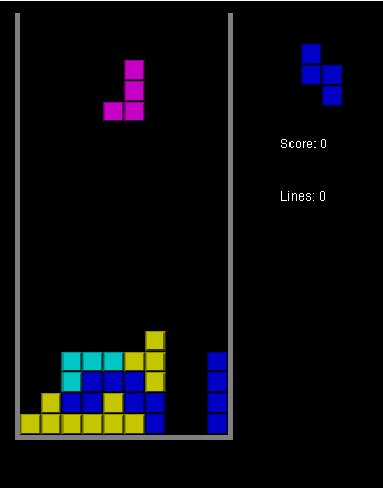
\includegraphics[width=2in]{tetgame.jpg}
\caption{Tetris game in progress}
\label{fig:tetgame}
\end{figure}

Tetris is so well established that it's name has basically lent itself to any entire genre of puzzle games.

 All variations have a range of different tetrominoes (see Figure \ref{fig:pieces} for examples), which are each defined by a static arrangement of square blocks. These tetrominoes can be rotated and translated in the absence of obstructions. 
 
A  single tetromino is selected by the game and appears in the top centre block of a fixed sized discrete well. The tetromino descends at a discrete fixed rate, that is determined by the current difficultly level, until it meets an obstruction. The tetromino is fixed in place if the contact still exists in the descent step following initial contact with an obstruction. If in being fixed it completes a row, the row is completely removed and the entire well contents above the deleted row are shifted downwards one row.

Many different artificial intelligence approaches have been applied to Tetris, and in order to remove implementation discrepancies in gauging the success of the relative algorithms, guidelines defining the Tetris game must be adopted. The agent, given the successful application of reinforcement learning, will therefore achieve results which will be directly comparable with those attained by other implementations following the same specifications. The standards set forth by \cite{tetstand} were selected as there is a fair amount of existing Tetris AI research associated with them and they seem reasonable, intuitive and comprehensive.

\subsection{Formal Tetris Specification \citep{tetstand}} 
\begin{itemize}
\item{Tetris has a board with dimensions 10 x 20}
\item{Tetris has seven distinct pieces (See Figure \ref{fig:pieces})}
\item{The current game piece is drawn from a uniform distribution of these seven pieces}
\item{Points are awarded for each block that is landed (not for completing rows)}
\item{The player scores the most points possible for each piece by executing a drop before one or more free-fall iterations transpire}
\item{The game has ten different difficultly settings, which determine the period of free-fall iterations, and are applied as row completion passes certain thresholds}
\end{itemize}

\begin{figure}[h]
\centering
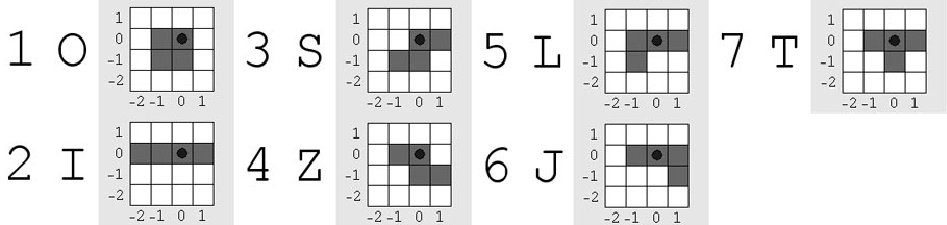
\includegraphics[width=\textwidth]{tetrisblocks.jpg}
\caption{The range of complete Tetris pieces as defined by \cite{tetstand}}
\label{fig:pieces}
\end{figure}

\subsection{Mathematical foundations of Tetris}

It has been mathematically proven \citep{mathproof,losetetris} that it is possible to generate a sequence of tetrominoes that will guarantee the eventual termination of any game of Tetris played in a well of width 2(2n+1), with n being any integer. This is most readily achieved by sending alternating Z and S pieces to the player, which lead to the gradual accumulation of persistent blocks and eventually the termination of the game \citep[Chpt. 5]{mathproof}. The implication of this is that even were the agent to play a flawless game of Tetris, over a long enough duration of play (infinite period), the series of tetrominoes that guarantee termination of the game are statistically inevitable.

Tetris has been proven to be NP-complete \citep{hardtet}. The implication of this is that it is computationally impossible to linearly search the entire policy space, and select an ideal action. This justifies the use of approximating techniques like reinforcement learning, in trying to determine the optimal policy.

One of the assumptions reinforcement learning requires is that the environment has the Markov property\citep{suttonbarto}. Tetris satisfies this requirement, as all the relevant information required to make an optimal decision is represented in the state at any instant in time. Rephrased, there is no historical momentum to the current state of the system, and any future occurrence is therefore entirely dependent on the current state of the system. If you are handed control of a Tetris games at any point, you are as equipped to play from that point as you would be had you played up until that point.

\section{Solving NP-Complete problems}

Attractive solutions to problems outside of the computational range of linear search methods can be discovered by emulating biological processes. Two such approaches are gentic algorithms and reinforcement learning. 

Genetic algorithms search directly in the solution (policy) space of a problem, breeding solutions amongst the fittest individuals in order to approach an optimal solution. Reinforcement learning yields an environment to an entity which is subsequently left to explore for itself, getting feedback directly from the environment in the form of rewards or penalties, and continuously updating its value function towards the optimal policy. Both methods ideally converge on the best policy\citep{evvsrl}, although their different routes gear them towards distinct problems. Reinforcement learning offers a higher resolution than genetic algorithms as genetic algorithms select optimal candidates at the population level while reinforcement learning  selects optimal actions at an individual level\citep{evvsrl}. Every action taken under a reinforcement learning policy is judged and driven towards the optimal action in that state, whereas in contrast genetic algorithms reward complete genetic strains, regardless of the behaviour of individual genes within the previous episode. Reinforcement learning also differs from genetic algorithms by indirectly adjusting it's policy through the updating of it's value function. 

A great deal of information is conveyed in the course of a Tetris game, and reinforcement learning would enable the agent to capture this information and adapt within the context of the game itself. This would also enable a directed real-time adjustment of the agents policy, rather then a global adjustment at the end of the game. 

These traits indicate a predisposition on the part of reinforcement learning towards a problem like Tetris.

\section{Reinforcement learning}
\subsection{Theory}

ACM Classification System (1998) I.2.8 Problem Solving, Control Methods, and Search

Reinforcement learning defines an approach to solving problems rather than specifying all the intricacies involved in solving the problem through to implementation. It is defined in terms of an agent interacting with an environment. The agent's perception of the environment is encapsulated in a value function which spans every state the environment can exist in, and associates an accumulative value with each of these states. This value function is updated upon receiving feedback, defined by the reward function, from the environment. This reward function is statically declared at the outset of a problem and is outside of the influence of the agent, and therefore steers the development of the value function. It is important to note that rewards can be either negative or positive, discouraging or encouraging the agent accordingly. The agent follows a policy that maps states to actions, and collaborates with the value function in dictating the behaviour of the agent\citep{suttonbarto}.

The goal of the agent is to maximise long term cumulative reward. Its initial behaviour is purely trial and error driven, but as the agent starts to form an impression about the states, and their relative merits, it becomes increasingly important for it to strike a balance between the exploration of new states which may provide maximum reward, and the exploitation of existing knowledge\citep{suttonbarto}.

Reinforcement learning can be applied in non-deterministic environments, where taking a certain action within the context of a state does not necessary lead to the same reward or same state transition. It does, however, require that the environment be stationary and that the probabilities of getting a certain reward or transitioning to a certain state remain the same\citep{kaelbling96reinforcement}.

At the core of every reinforcement learning problem is the value function. In its most simple form this would be a table containing a value for every state. These values are an indication of the long term reward associated with a particular state. The value function is continually adjusted using equation \ref{eq:sarsa}. 

\begin{eqnarray}
\centering
V(s_t) & \leftarrow & V(s_t) + \alpha(r_{t} + \gamma V(s_{t+1}) - V(s_t)) \label{eq:sarsa}
\end{eqnarray}

$V(s_t)$ refers to the value of the current state, $V(s_{t+1})$ refers to the value of the next state and $r_t$ refers to the reward received in transitioning from the current state to the next state. 

The $\alpha$ and $\gamma$ terms dictate the behaviour of the update function. 

The $\alpha$ term determines the weighting of the current adjustment in relation to all previous adjustments. A large constant $\alpha$ gives recent value function adjustments a larger influence then historical adjustments. In order to guarantee convergence this $\alpha$ value must be kept relatively small, and this can be further guaranteed by having the $\alpha$ value diminish over the course of an agents training. 

The $\gamma$ factor determines the extent to which future rewards affect the current value estimation. The larger the $\gamma$ term, the greater the significance attributed to future rewards. This approach of "backing up" the values is an example of temporal-difference learning\citep{suttonbarto} and is a way of propagating information about future rewards backwards through the value function.

Equation \ref{eq:sarsa} states that the value associated with the current state is equal to the current value and a correction factor. This factor is the difference between the sum of the observed reward and discounted future rewards, and the current states value. The value function therefore incrementally converges to an optimal solution.

The agent can possess one of a variety of policies. With a purely greedy policy, the agent will always select the state transition believed to offer the greatest long-term reward. Although this will immediately benefit the agent, it may well fail to find the ideal policy in the long run. With an $\epsilon$-greedy method the agent will select the best state transition the majority of the time and take exploratory moves on all the other state transitions. The frequency of these exploratory moves is determined by the value of $\epsilon$ utilised by the policy. It is possible to vary $\epsilon$, in order to have an initially open minded agent that gains confidence in its value function as its experience increases over time. One problem inherent in the $\epsilon$-greedy approach, is that the agent explores indiscriminately and is as likely to explore an obviously unattractive avenue as it is to explore a promising one. An alternative approach is offered by the softmax approach shown in equation \ref{eq:softmax}. This associates a probability of selection with every possible transition, which is proportional to the the predicted value of that transition. This encourages the agent to explore promising looking transitions more thoroughly then less promising ones.

\begin{eqnarray}
\centering
P & = & \frac{e^{Q_{t}(a)/\tau}}{\Sigma_{b=1}^{n}e^{Q_{t}(b)/\tau}} \label{eq:softmax}
\end{eqnarray}

The degree to which the estimated value effects the probability of selection is varied by the $\tau$ term, which is referred to as the temperature. For large temperatures the state transitions become almost equiprobable, while at low temperatures the probabilities spread out according to the strength of the value function. In the limit as temperature goes to zero, the policy converges to the greedy policy.

When a goal has been reached the reward function yields a reward to the agent.  The value  associated with the originating state is incremented accordingly and is backed up throughout the value function in the course of the following transitions\citep{suttonbarto}.

The value function does not necessarily have to take the form of a table. The value function can be seen as a mathematical function that takes the originating state as input and outputs the state with the highest predicted value. Rather then storing the values in a table, the information is stored in the behaviour of the function.

\subsection{Existing applications}

Reinforcement learning performs very well in small domains and by using the insight offered by \cite{suttonbarto} it is fairly simple to create an agent that plays simple games like Tic-Tac-Toe or Blackjack successfully. It has been successfully applied to many sophisticated problems such as :

\begin{itemize}
\item{Packet routing in dynamically changing networks \citep{boyan94packet}}
\item{Robotic control \citep{rlrobotics}}
\item{Acrobot \citep{suttonbarto} }
\item{chess \citep{baxter98knightcap}}
\end{itemize}

Bellman is cited \citep{suttonbarto} as stating that reinforcement learning suffers from the "curse of dimensionality".  This refers to the exponential increase in the complexity of the system, as the number of elements in it increase linearly. This tendency has resulted in relatively few successes in large state-space domains\citep{keepaway}. These successes include 

\begin{itemize}
\item{Robo-Cup Keep-Away \citep{keepaway}}
\item{Backgammon \citep{tdgammon}}
\item{Elevator control \citep{elevator}}
\item{Helicopter control}
\end{itemize}

\subsection{Large state-space successes}

\subsubsection{TD-Gammon}

 \cite{tdgammon} used reinforcement learning to train a neural network in playing Backgammon. The program was so successful that its first implementation (Version 0.0) had abilities equal to Tesauro's well established Neurogammon\footnote{Neurogammon was a neural network backgammon player, trained on a database of recorded expert games, who convincingly won the 1989 International Computer Olympiad backgammon championship.} \citep{tdgammon}.  More noteworthy is that by Version 2.1 TD-Gammon was regarded as playing at a level extremely close to equalling that of the worlds best human players, and had even started to influence the way expert backgammon players played\citep{tdgammon}. The unbiased exploration of possible moves, and reliance on performance rather then established wisdom led, in some circumstances, to TD-gammon adopting non-intuitive policies superior to those utilised by humans\citep{tdgammon}.

Backgammon is estimated to have a state space larger then $10^{20}$. This state space was reduced by the use of a neural network organised in a multilayer perception architecture. Temporal difference learning, with eligibility traces, was responsible for updating the weighting functions on the neural network at the game progressed. Another perk associated with using reinforcement learning methods rather then pure supervised learning methods, was that TD-gammon could be (and was) trained against itself\citep{tdgammon}.

\subsubsection{RoboCup-Soccer Keep-Away}
\cite{keepaway} managed to successfully train reinforcement learning agents to complete a subtask of full soccer which involved a team of agents, all learning independently, keeping a ball away from their opponents. 

This implementation overcame many difficulties, such as having multiple independent agents functioning with delayed rewards and most importantly, functioning in a large state space. The state space problem was resolved by using linear tile-coding (CMAC) function approximation to reduce the state space to a more feasible size\citep{keepaway}.

\subsection{Tetris}

\subsubsection{\cite{melaxtetris}}

Melax set out to apply reinforcement learning to a greatly reduced version of the Tetris game. His Tetris game had a width of six, a well of infinite height and a greatly reduced piece set. The length of the game was therefore dictated by the number of tetrominoes attributed to a game and was set at 10000. Although the height of the Tetris well was infinite in theory, the active layer in which blocks could be placed was two blocks high, and any placement above this level would result in the lower layers being discarded until the structure had a height of two. The game kept a record of the number of discarded rows and this was used as a score for the performance of the agent. This approach to scoring resulted in better performance corresponding to a lower score. 

The two block active height prevented the agent from completing rows he was previously incapable of filling. This differs from traditional Tetris where a player can complete an unfilled row upon reducing the well structure down to it. Since the pieces are assigned stochastically and unfilled rows form an inexorable blemish on the performance measure of the agent, this introduced a random aspect to the results.

The agent was implemented using tabular sarsa, and was punished a hundred points for every level it introduced above the working height of the well.

Melax's agent achieved significant learning, as shown in table \ref{mresults}. These results are reflected in figure \ref{fig:meres}.

\begin{table}[h]
\centering
\begin{tabular}{|r|r|}
\hline
Game & Height  \\
\hline
    1 &  1485 \\
     2  & 1166 \\
     4  & 1032 \\
     8  &  902 \\
    16  &  837 \\
    32  &  644 \\
    64  &  395 \\
   128  &  303 \\
   256   & 289 \\
\hline
\end{tabular}
\caption{Melax's results for reduced Tetris}
\label{mresults}
\end{table}

\begin{figure}[h]
\centering
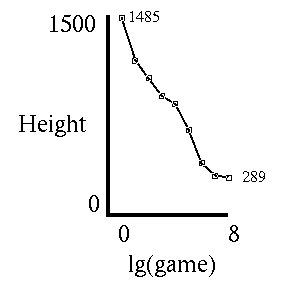
\includegraphics[width=2in]{melaxresults.png}
\caption{Melax's results as taken from \cite{melaxtetris}}
\label{fig:meres}
\end{figure}

As the number of games increased, the agent learnt how to minimise the total height of the pieces in the well and therefore maximised its long term reward.

One possible problem with this implementation is that by defining rewards for sub-goals, such as increasing the working height, Melax was effectively steering the development of the agent's policy. Keeping the height of the game low tends to extend the life of the agent and entails the completion of rows since the agent avoids building vertically. This might actually be the ideal policy for the agent to adopt, especially in the context of our adopted Tetris specifications \citep{tetstand}, but our agent has just lost one potential avenue of exploration. 

\subsubsection{\cite{yaeltetris}}

Melax's approach was adopted by Bdolah \& Livnat, who investigated different reinforcement learning algorithms and introduced state space optimisations. The state space was reduced through two distinct approaches. In the first approach, subsurface information was discarded leaving only the contour of the game for consideration. This approach was further divided into either considering the contour differences as either being positive or negative, or reducing the height differences to a small spectrum of height differences. The second state space reduction made use of mirror symmetry within the well in order to reduce the number of different states. This functioned within Melax's original representation of a well with two block active height.

\begin{figure}[h]
\centering
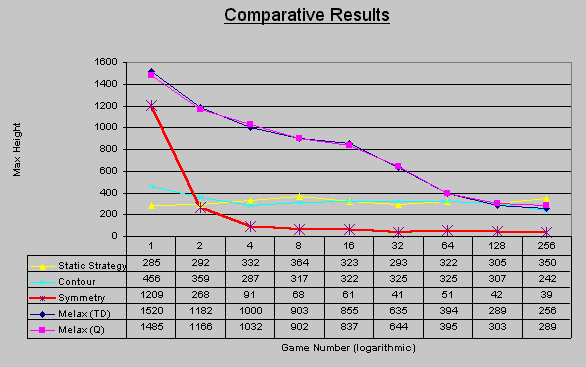
\includegraphics[width=2in]{results.png}
\caption{Bdolah \& Livnat's results as taken from \cite{yaeltetris}}
\label{fig:yaelres}
\end{figure}

Both optimisations appear to have greatly improved the performance of the agent, judging by the chart shown in figure \ref{fig:yaeltres}. The are however some troubling aspects to these results.

The mirror symmetry results are far superior to the results achieved by any other method. As mentioned earlier, this optimisation made use of redundancy in the active block height of two used by Melax. This optimisation effectively ignored one reflection of duplicated states, and thus should have sped up the learning process, but converged to the same solution. The accelerated learning is evident but the results indicate that the mirror symmetry actually led to the adoption of a distinctly different policy to that adopted by the agent with separate mirrored value entries.   

The contour learner extended the perceptions of the agent, and maintained the information pertenant to levels below the original two layer structure. This enabled the agent to continually reduce the well structure of the course of the game, and reduce gained height. These results seem to indicate incredibly fast learning. By the end of the first game the agent has settled on a policy that produces a result far in advance of the original Melax result, however the results then plateau. 

\subsubsection{\cite{kurt}}

Relational reinforcement learning was applied to the full Tetris problem by \cite{kurt}. Relational reinforcement learning differs from traditional methods in the structuring of the value function. Rather then storing every possible state in a table, the relationship between the elements in the environment is utilised in developing a reduced state space. This state information is then stored in a decision tree structure. 

Driessens approached the problem with three separate relational regression methods \citep{kurt} he had developed over the course of his thesis. The first of these regression methods had already proven itself in the course of the thesis with the successful extension of reinforcement learning to Digger\footnote{Another game with a large state space}. 

Driessens results are shown in table \ref{tbl:driessens} .

\begin{table}[h]
\centering
\begin{tabular}{|r|r|r|}
\hline
Regression method & Learning games & Completed rows  \\
\hline
RRL-TG	&	5000	& 	10   \\
\hline
RRL-RIB  &  50  & 12  \\
\hline
RRL-KBR  &  10-20  & 30-40  \\
\hline
\end{tabular}
\caption{Relational regression results \citep{kurt}}
\label{tbl:driessens}
\end{table}

The RRL-RIB reached its optimal policy within 50 training games. In 450 subsequent training games this policy was not improved upon. RRL-KBR reached a better policy, earlier then the other regression methods. It then rather unexpectedly unlearnt its policy after a further 20-30 learning games.

Since this is actually a full implementation of Tetris it can be compared against other AI results, where the best (comparable) methods score in the region of 650 000 completed rows\citep{tetstand}. These results are not impressive in the light of the competition, and very poor even by human standards. 

Driessens attributes the poor functionality to Q-learning, stipulating that Q-learning requires a good estimate of the future rewards in order to function properly and that the stochastic nature of Tetris severely limits the accuracy of these estimates. Since his regressions methods were derived from Q-learning, this inadequacy impacted on all of his methods. Q-learning in known to be unstable\citep[pg. 4]{keepaway,thrun93issues} when incorporated in function approximation, and this could certainly have contributed to the poor performance witnessed in the above results.

\chapter{Design}

\section{Overview}

The design of the system was broken into three distinct areas. We had to consider the structure of the application as a whole in order to make it as modularised as humanly possible. We had to consider the reinforcement methods we were intending to implement and how they would interface with the Tetris game. We had to consider the Tetris state space and suggest simplifications that would reduce the amount of redundant information the system had to deal with. 

\section{Application design}

\subsection{The investigation platform}

We designed a Tetris game from first principles in order to have complete control over the structure of the game, and familiarise ourselves with the methods required by a Tetris game.

The game can be readily divided up into the following logical classes.

\begin{itemize}
\item{The game window}
\item{The Tetris game}
\item{The tetromino set}
\item{The tetromino object}
\item{The reinforcement learning agent}
\end{itemize}

The interaction between these components is shown in figure \ref{fig:uml}

\begin{figure}[h]
\centering
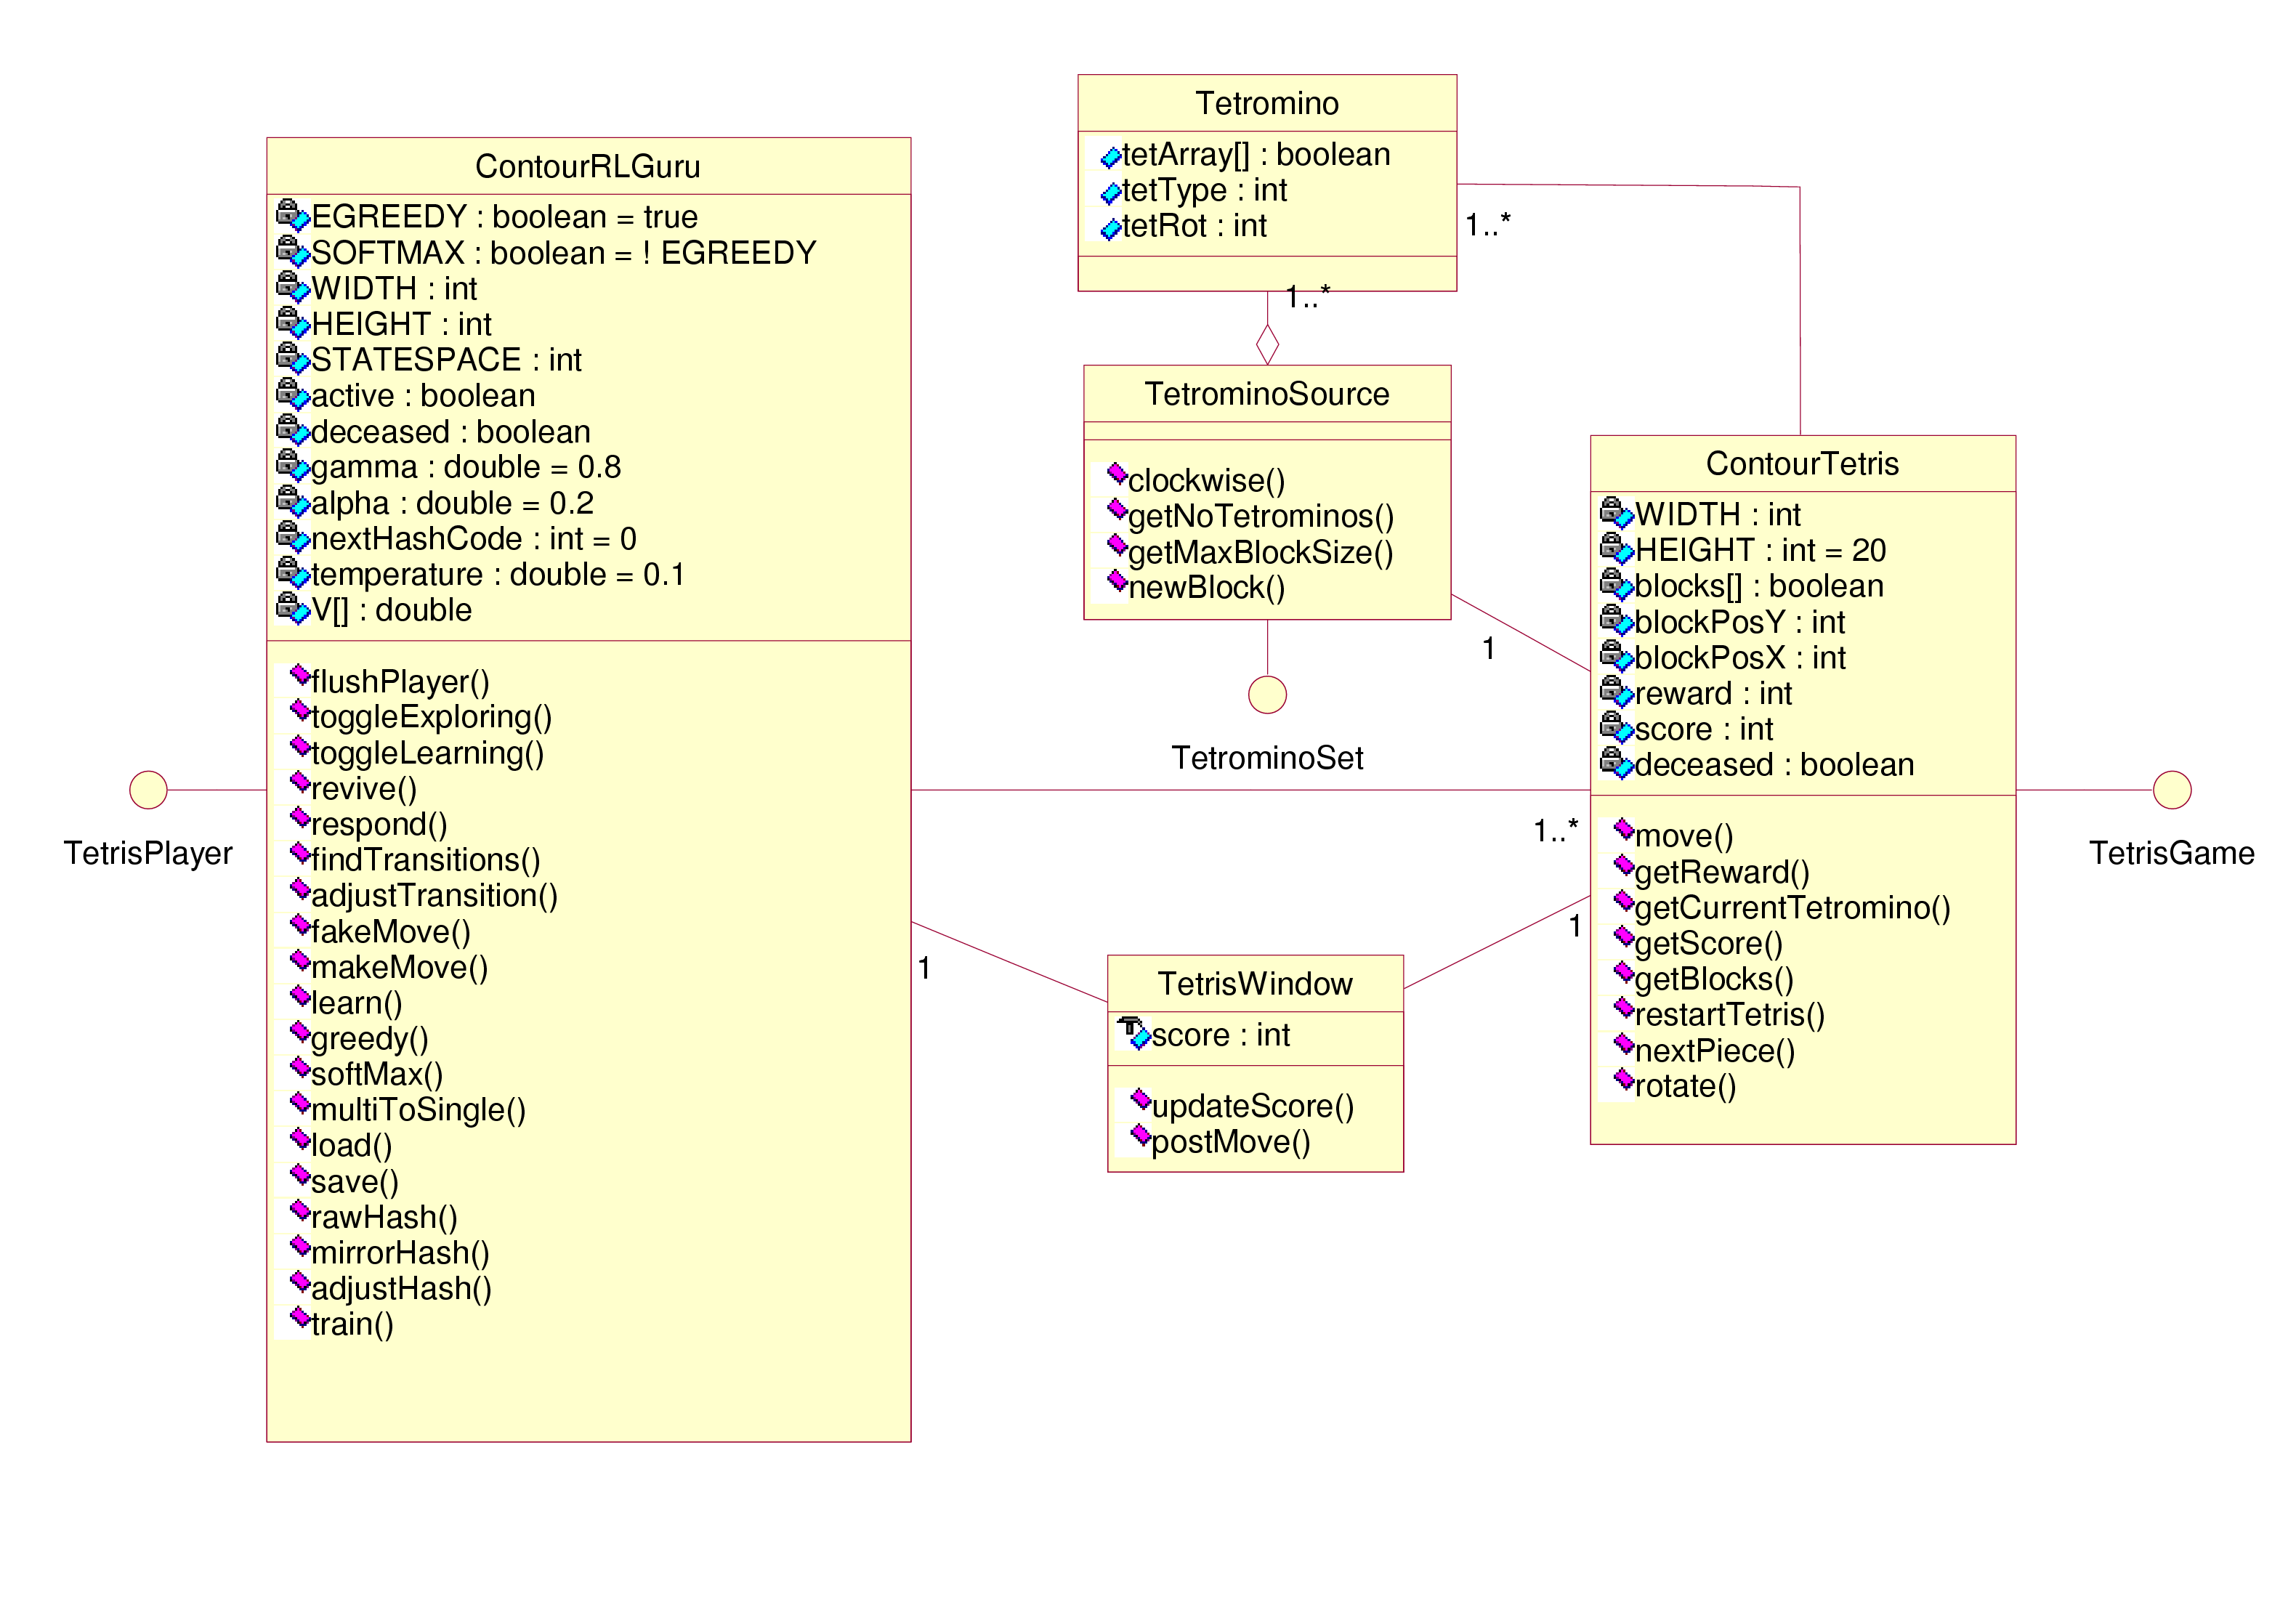
\includegraphics[width=6in]{finaluml.png}
\caption{Class diagram of reinforcement learning orientated Tetris}
\label{fig:uml}
\end{figure}

The game window acts as the interface between the user and the Tetris game, and is responsible for displaying all information regarding the system. The Tetris game is the self contained core of the program and is responsible for managing the game and yielding information on the state of the game. The Tetris game and agent are both instantiated in the game window and the agent passed a reference to the game upon instantiation. Exclusive control is switched between either of these two control sources and the game is therefore oblivious to the source of its instructions.  Including human interaction enables the Tetris implementation to be checked. The tetromino set is instantiated within the Tetris game, and is responsible for the definition and rotational manipulation of the tetrominoes. All tetromino transitions which occur within the well are checked and performed in the Tetris game. The tetromino object is common to all methods, and is a simple structure encapsulating the traits of the Tetromino. This object is oblivious to the definitions dictated by the tetromino source, and is used by all the classes.

The Tetris game, tetromino set and the artificial agent are all objects that will need to change in the course of the investigation. This is simple if these three objects implement generic interfaces and therefor allow us to utilise polymorphism. This structuring allows for seamless swapping between different game definitions, tetromino sets and artificial agents. The differing game definitions are largely restricted to variations in the dimension of the well. The tetromino definitions are unrestricted and any tetromino collection can be created. As long as the agent implements correct interface, the theory guiding the actions of the agent can subscribe to any artificial intelligence method.

\subsection{Fly-weight design pattern}

We would expect any object orientated Tetris game to deal with a large number of tetromino objects. The performance penalty introduced by instantiating millions of objects warrants consideration and is addressed by conventional design patterns. 

Rather then having the game continually recreating individual tetrominoes within the set of available tetrominoes, it is possible to create every possible tetromino once and subsequently pass out a reference to the relevant tetromino. This corresponds to a fly-weight design pattern, as discussed in \cite{designp}, and removes the overhead associated with instantiating numerous simple objects.

The implementation is piece specific and is therefore defined in the tetromino source class. In this class an two dimensional array of tetrominoes is instantiated with dimensions dictated by the number of different tetrominoes and the number of orientations. The first time an object is assigned or rotated it is created within this array structure. Once the table is constructed, assigning a tetromino sets the array within a sub-array of four tetrominoes on the default rotation. If a rotation request succeeds the rotation index is altered accordingly, and this pointer returned.

\subsection{Designing the agent}

We set out to create an agent with no look ahead, and therefore only the tetromino currently allocated to the agent is considered during each move.

We decided to experiment with afterstates and sarsa learning, which utilise equation \ref{eq:astates} \& \ref{eq:sarsa2} respectively.

\begin{eqnarray}
\centering
V(s_t) & \leftarrow & V(s_t) + \alpha(r_{t} + \gamma V(s_{t+1}) - V(s_t)) \label{eq:astates} \\
Q(s_t,a_t) & \leftarrow & Q(s_t,a_t) + \alpha(r_{t} + \gamma Q(s_{t+1},a_{t+1}) - Q(s_t,a_t)) \label{eq:sarsa2}
\end{eqnarray}

We also decided to experiment with three different exploration methods, namely

\begin{itemize}
\item{Optimistic exploration}
\item{$\epsilon$-greedy}
\item{softmax}
\end{itemize}

\section{Redesigning the state space}

Traditional reinforcement learning uses a tabular value function, which associates a value with every state. Since the Tetris well has dimensions twenty blocks deep by ten blocks wide, there are 200 block positions in the well that can be either occupied or empty.

\begin{figure}[h]
\centering
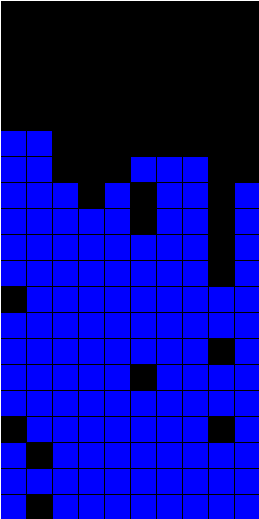
\includegraphics[width=0.8in]{fullwell.png}
\caption{The complete Tetris well}
\label{fig:fullwell}
\end{figure}

\begin{eqnarray}
\centering
\textrm{State Space} & = & 2^{200} 
\end{eqnarray}

This is an unwieldy number and since a value would have to be associated with each state, this representation is completely non-feasible. By considering the game from a human perspective, we considered some practical reductions in state space. 

\subsection*{Assumption 1}

The position of every block on screen is not a consideration that is factored into every move. We only consider the contour of the well when making decisions. We limit ourselves to merely considering the height of each column.

\begin{figure}[h]
\centering
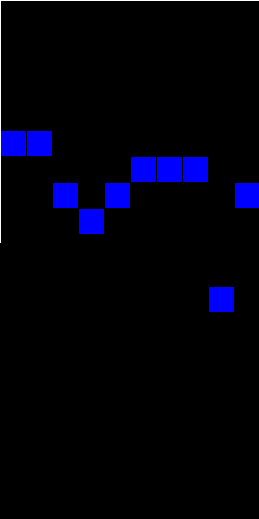
\includegraphics[width=0.8in]{heightwell.png}
\caption{Height based Tetris well}
\label{fig:heightwell}
\end{figure}

\begin{eqnarray}
\centering
\textrm{State Space} & = & 20^{10} \approx 2^{43}
\end{eqnarray}

\subsection*{Assumption 2}

The height of each column is fairly irrelevant except perhaps when the height of a column starts to approach the top of the well. Ignoring this for the time being, the importance lies in the relationship between successive columns, rather then their isolated heights.

\begin{figure}[h]
\centering
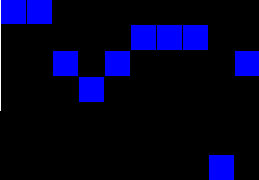
\includegraphics[width=0.8in]{diffheightwell.png}
\caption{Height difference based Tetris well}
\label{fig:diffheightwell}
\end{figure}

\begin{eqnarray}
\centering
\textrm{State Space} & = & 20^{9} \approx 2^{39}
\end{eqnarray}

\subsection*{Assumption 3}

Beyond a certain point, height differences between subsequent columns are indistinguishable. A human will not adopt different tactics when the height difference between two columns advances from nineteen to twenty. We could either cap the maximum height differences, or start separating the heights into fuzzy sets as the height differences increase past certain thresholds. We cap the maximum height difference between wells as $\pm$ 3, and round all height differences outside of this range down to $\pm$ 3. The agent will therefore generalise for any height difference greater then 3. Since only the straight tetromino can span a height difference of 3, and this tetromino can span any height difference, this assumption seems fair to make. 

\begin{figure}[h]
\centering
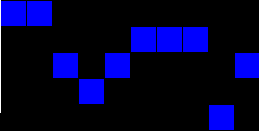
\includegraphics[width=0.8in]{capdiffheightwell.png}
\caption{Capped height difference based Tetris well}
\label{fig:capdiffheightwell}
\end{figure}

\begin{eqnarray}
\centering
\textrm{State Space} & = & 7^{9} \approx 2^{25}
\end{eqnarray}

\subsection*{Assumption 4}

The largest tetromino is four blocks wide. At any point in placing the tetromino, the value of the placement can be considered in the context of a subwell of width four. These subwells could then be reproduced across the extent of the full well.

\begin{figure}[h]
\centering
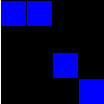
\includegraphics[width=0.8in]{reducedwell.png}
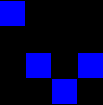
\includegraphics[width=0.8in]{reducedwell2.png}
\caption{Capped height difference based Tetris subwells}
\label{fig:redwell}
\end{figure}

\begin{eqnarray}
\centering
\textrm{State Space} & = & 7^{3} = 343 \approx 2^{8}
\end{eqnarray}

\subsection*{Assumption 5}

Since the game is stochastic, and the tetrominoes are uniformly selected from the tetromino set, the value of the well should be no different to its mirror image.

\begin{figure}[h]
\centering
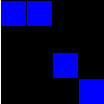
\includegraphics[width=0.8in]{reducedwell.png}
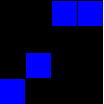
\includegraphics[width=0.8in]{mirrorwell.png}
\caption{Mirror identical states}
\label{fig:mirrorwell}
\end{figure}

\begin{eqnarray}
\centering
\textrm{State Space} & = 175
\end{eqnarray}

We now have a much reduced statespace, which we hope will neither limit the player nor appreciably steer its policy. The implications of the assumptions should be considered before we progress.

Assumption 1 discards all information about the subsurface structure of the well. The initial representation can be perceived to store the location of every hole in the structure. The agent will therefore be oblivious to any differences between transforming to a said contour and the same contour with spaces beneath the surface. The existing holes are not important, but we may wish to include a penalty for the holes introduced during a state transition.

Assumption 2 introduces no obvious evils.

Assumption 3 removes the agents ability to distinguish between extremes in height differences.

Assumption 4 removes the global context in which the agent functions, and restricts his view to each individual transition. We may need to dynamically reestablish the context in which he is functioning.

Assumption 5 reduces the state space in a non-simple fashion. The mirrored states are still allocated space, but are never explored, removing the computational burden they represent. 


\chapter{Implementation}

The various exploration algorithms can be applied across any reinforcement learning method. It therefor makes sense to divide the various steps into discrete methods.

Optimistic learning is achieved by initialising the value function with values slightly larger then the largest anticipated value. This value is easily determined when dealing with purely negative rewards, since all states will have negative values. When dealing with positive rewards, the easiest approach is to set the agent to explore for a large period of time, look at the predicted values and adopt a value slightly larger then the largest value for the starting values.

The agent uses a hashing function in order to associate a state with a position in the value table. The hashing function is completely dependent on the state representation of the game.

For the Melax type agent the well is viewed as a 12 block array. The first position is assigned a value of one and this value is doubled for each successive block position. If the position is occupied, the value of that position is added to a floating sum. This enables us to calculate a unique hash code for every state through the use of addition.

For our reduced well agent the well is viewed as a block array one block narrower then the game the agent is playing in. Each of these positions can have a value between 0 and 6, corresponding to a height difference of -3 and 3 accordingly. The first position is assigned an intrinsic value of 1. The intrinsic value of each subsequent position is determined by multiplying the previous positions intrinsic value by 7. Multiplying the values in the block array by the intrinsic value of the array position and summing the resulting products yields a unique hashcode. This method is not limited to height differences of 7, and is readily expandable with the inherent values of the block positions increasing as $x^n$, where x is the number of height differences and n the relative row position.

Mirror symmetry is achieved in both of the above hash functions by calculating the hash codes from both directions. The smallest value is then always selected. The unused hash codes are still issued storage space, but are never explored and therefore introduce no exploratory overhead.

The above hash functions solve the problem of representing the state space. Expanding the agents perception beyond the state is handled by introducing a adjustment to the previous hashCode. This adjustment hash function adds further weighted terms to the existing hash code. The weighting used is always the full size of the previous state description. Sarsa for instance requires state-action value tables. The state hash function is adjusted to include the tetromino type, position of placement and number of rotations. Each enhancement adds the existing hash code to the new consideration multiplied by the existing state space. 

The agent possesses a method for discovering the available transitions from the current state. This method makes use of a virtual game that exists purely for the benefit of the agent. The agent transposes the block formation from the real Tetris game into his virtual well and then proceeds to perform each of the possible transitions individually within the virtual well. Each of these transitions is hashed to discover the associated value.    

$\epsilon$-greedy and softmax are implemented as competing exploration methods, with either of them functioning alongside optimistic learning if desired. Both methods accept a range of possible transitions and return a single transition.x
 
The reduced wells comprising the full well are related to the full well by a transition adjustment function. The same transition exists across the various wells, and these subtransitions are manipulated to reflect the unique value of a transition in the full well. This can be achieved in a variety of ways, each of which lend a strong influence to the final result. The sub-transitions can be averaged, leading to a single transition which reflects the value of the transition across all the subwells and gives a broad overview of the value of the transition. Another approach is to retain the lastest transition value from all the subwells. This singles out the largest transition and disregards all other transitions, placing the emphasise on selection the optimal action over all others.

The afterstates method only factors the value of the destination state in considerations. This value represents the long term value stemming from a state, and is completely ignorant of the transition between the current state and the destination state. This leads the agent to be obsessive about states and always transition to states that promise future reward, even if the transition bypasses immediately available reward. It is therefore possible for an agent which has converged on the optimal policy to still display no clear reasoning and perform terribly. The combination of the immediate reward associated with a transition and the value of the destination state bypasses the problem. This leads the agent to consider both the long and short term behaviour of the system, although it breaks with the idea of an agent who converges on a term representative of short and long term reward.
 
The sarsa method identifies every transition leaving a state, and thereby focuses on the transitional values neglected by the afterstates player.

\chapter{Melax player}

\section{Introduction}

My first goal was to experiment with reinforcement learning and to reproduce Melax's learning results in my implementation of Tetris.  

Melax clearly defined the conditions under which his player functioned

\begin{itemize}
\item{Well has infinite height}
\item{Well has width of 6 blocks}
\item{The game has a working height of 2 blocks : Any blocks below this are discarded}
\item{The game has 10000 tetrominoes}
\item{The alpha and gamma values are defined as 0.02 and 0.8 respectively}
\end{itemize}

Melax did not stipulate the exact reinforcement learning approach he applied to his agent, although the update function stated in \cite{melaxtetris} corresponds to an afterstates update function.

Optimistic learning was employed, and the initial value estimates for each state were set to zero, which is optimistic when receiving purely negative rewards.

We implemented an agent according to these stipulations.

\begin{figure}[h]
\centering
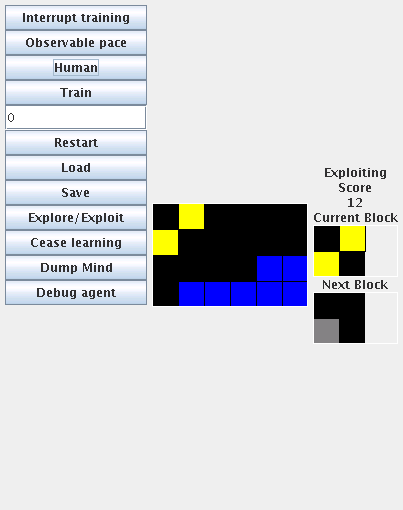
\includegraphics[width=3in]{mymelax.png}
\caption{Our Melax defined agent}
\label{fig:mymelax}
\end{figure}

\begin{table}[h]
\centering
\begin{tabular}{|r|r|r|}
\hline
	&	mirror	&	melax \\	
\hline
1	&	1607	&	1793	\\
\hline
2	&	1194	&	1493	\\
\hline
3	&	970	&	1203	\\
\hline
4	&	813	&	1103	\\
\hline
5	&	740	&	1040	\\
\hline
6	&	693	&	980	\\
\hline
7	&	667	&	877	\\
\hline
8	&	623	&	829	\\
\hline
9	&	605	&	712	\\
\hline
10	&	621	&	789	\\
\hline
11	&	600	&	720	\\
\hline
12	&	593	&	683	\\
\hline
13	&	605	&	598	\\
\hline
14	&	588	&	594	\\
\hline
15	&	586	&	652	\\
\hline
16	&	551	&	651	\\
\hline
17	&	590	&	604	\\
\hline
18	&	623	&	604	\\
\hline
19	&	547	&	608	\\
\hline
20	&	538	&	606	\\
\hline
\end{tabular}
\caption{Values of melax and mirror symmetry agent}
\end{table}

\begin{figure}[h]
\centering
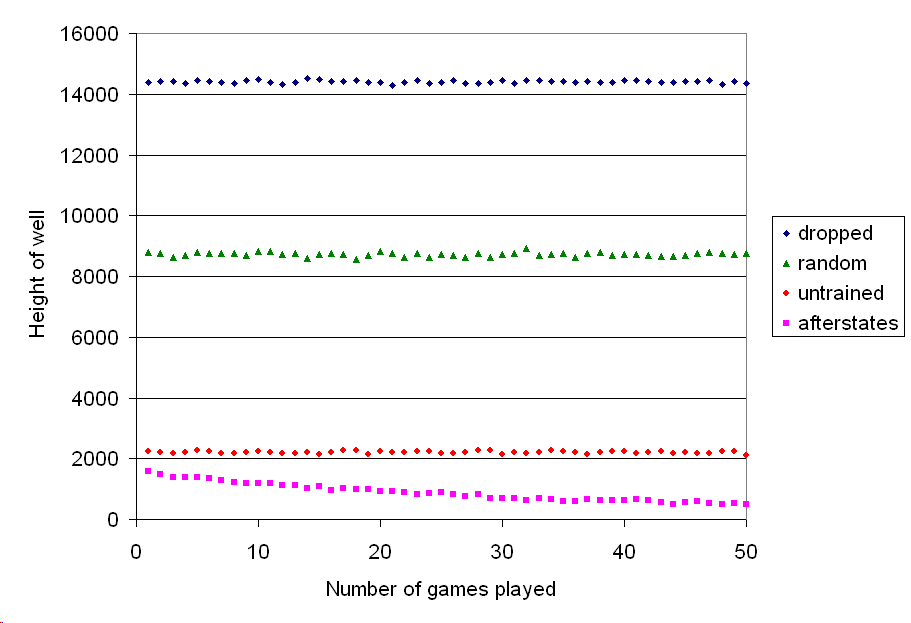
\includegraphics[width=3in]{mymelaxresults.png}
\caption{Results for the Melax defined agent}
\label{fig:mymelaxresults}
\end{figure}

The results shown in figure \ref{fig:mymelaxresults} contrast the performance of our reinforcement learning player to other standards. 

The first standard is the maximum height of the structure and is determined by piling up tetrominoes without undertaking any translation or rotation.

The second standard is the height of the structure when the blocks are randomly placed.

The third standard is the performance of the agent when he is set to exploit his knowledge, without the benefits of having been trained first. As can be seen the agent has a fair amount of insight into the game through the nature of the learning method. The afterstates method only associates a value with a state, and not with the transitions that lead to that state. The implication of this is that the agent will only be interested in the final state, and not the repercussions of transferring to that state. This means that an agent with the possibility of completing a row, may actually choose to increase the height of the structure, since the final state after the height increase has a lower chance of leading to a further height increase. This is circumvented by alerting the agent to the reward associated with a transition and the value of the destination state, when compiling the list of possibly transitions. This is the factor responsible for the impressive performance of the untrained agent.

The agent starts at the level of the untrained agent and rapidly improves. The height of the well stabilises at a height which is roughly a quarter of the height of the untrained agent.

We proceeded to implement the mirror symmetric optomisation of the Melax state space identified by\cite{yaeltetris}. Figure \ref{fig:comparemelax} shows the improvement in the agents performance when the mirror symmetry optimisation is included in the state description. Since all the mirror symmetrical states reference the same position in the table, these values are updated twice as often as they were before the optimisation. This leads to the tabular values converging on the correct values more rapidly. This is clearly reflected in the graphed results, and it is important to note that the final policy arrived at is the same in both circumstances. This vindicates the assumption that mirror identical states should have the same value associated with them.

\begin{figure}[h]
\centering
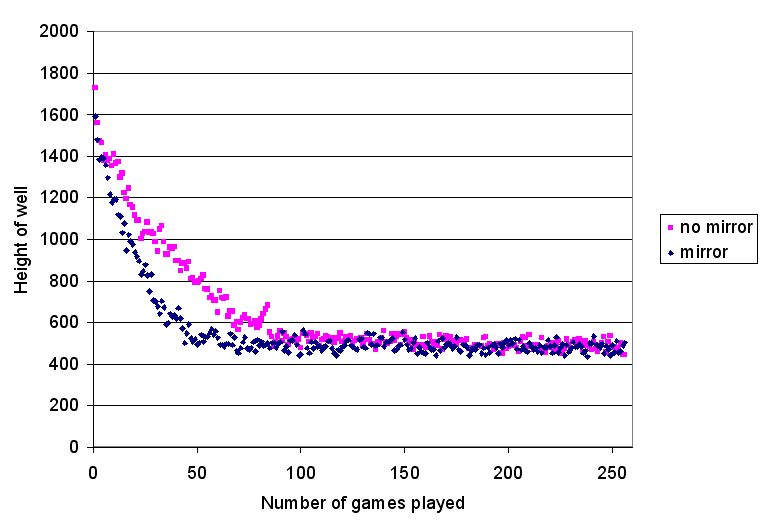
\includegraphics[width=3in]{mirrormelax.png}
\caption{Performance impact of mirror symmetry}
\label{fig:comparemelax}
\end{figure}

We used the Melax agent to compare the performance of the agent when using the different exploration methods. These results are shown in figure \ref{fig:comparelearning}. The $\epsilon$-greedy method explores 5 percent of the time. The softmax approach introduces difficulties, as it is difficult to ascertain a good initial temperature, rate of change of temperature and final temperature.

Melax mentions having implemented a sarsa agent and states that there was no appreciable differences in the results achieved by the agent. We implemented a sarsa agent to play the Melax Tetris game and the results are show in figure \ref{fig:melaxsarsa}.

\begin{figure}[h]
\centering
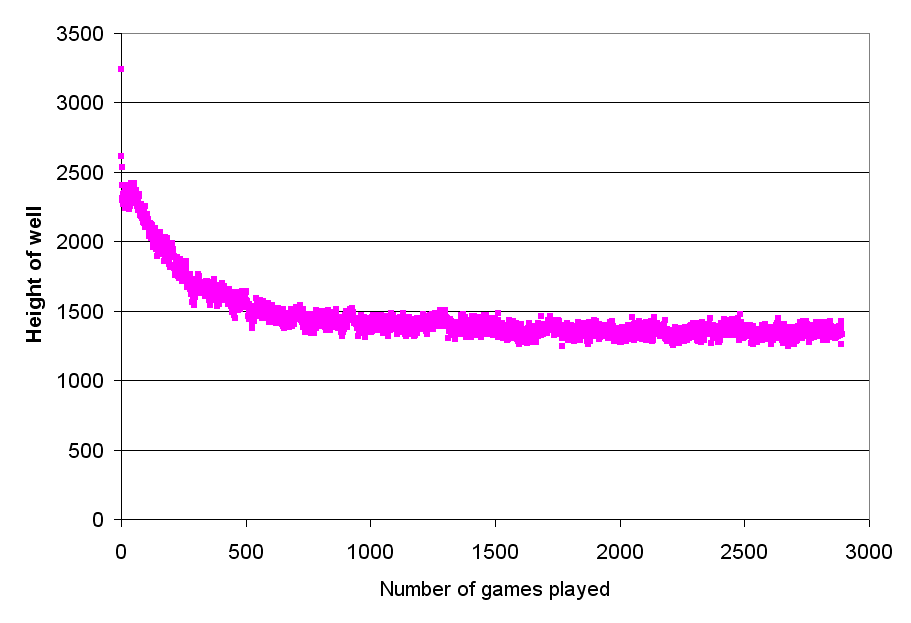
\includegraphics[width=3in]{sarsamelax.png}
\caption{Performance impact of mirror symmetry}
\label{fig:melaxsarsa}
\end{figure} 

The value table had to be extended to contain every transition off each state. The number of transitions is dictated by the number of different tetrominoes, the width of the well and the number of different orientations. Melax's reduced piece set contains 5 different tetrominos, the well is 6 blocks wide and any grid based game is restricted to 4 orientations. There are therefore approximately 5*6*4 transitions off each state and the size of the state space is increased from 4096 states ($2^{12}$) to 491520 states (approximately $2^{19}$). This introduces a large amount of redundent information since only the L shaped Melax tetromino has 4 unique orientations, while all the others only have 2 unique orientations. There is further storage wastage as only the single block tetromino can move across the full span of the well regardless of the orientation of the block. All these factors require piece specific consideration and incorporating them in our Tetris implementation would remove the generic nature of the implementation. Although this redundancy introduces additional training time, it should not impact on the final values converged on by the value function.

\chapter{Contour Player}

\section{Afterstates agent}

The afterstates agent performed well in a reduced well four blocks wide. As the width was increased the performance of the agent deteriated drastically. 

We experiment with several different reward policies. Initially we wanted to lead the player as little as possibly and afford if the freedom to determine its own policy. Melax's punishing of the agent for increasing the height seemed too perscriptive, and we initially opted to rather reward the agent for simply completing rows. This met with success when used with the afterstates agent however the sarsa player performed poorly due to the sparsity of rewards.

There were two obvious shortcomings to be seen in the performance of our original afterstates agent. The agent was oblivious to the introduction of holes and introduced them with gusto. We tried to correct for this by adopting a real time penalty for introducing covered holes. This introduced the problem of weighting the hole penalty against the  

In the sarsa player, the height of the well and the number of 
\begin{figure}[h]
\centering
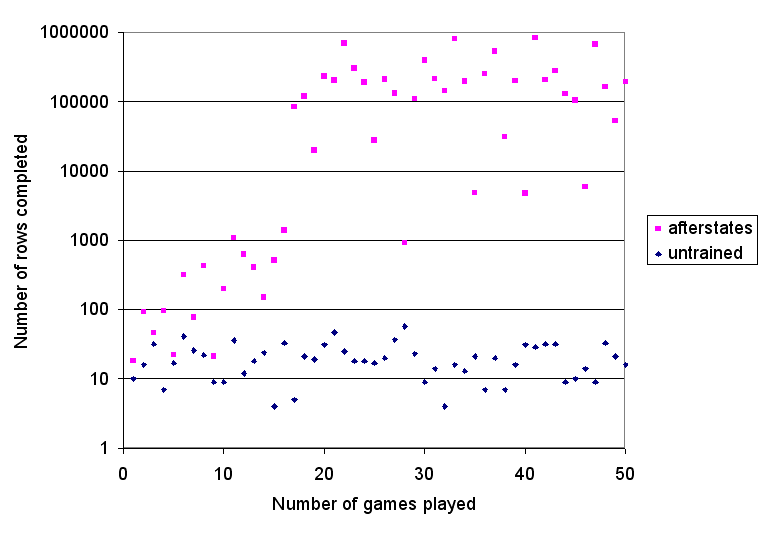
\includegraphics[width=3in]{afterstatesredtet4well.png}
\caption{Afterstates agent in well of width 4}
\label{fig:comparemelax}
\end{figure}

\begin{figure}[h]
\centering
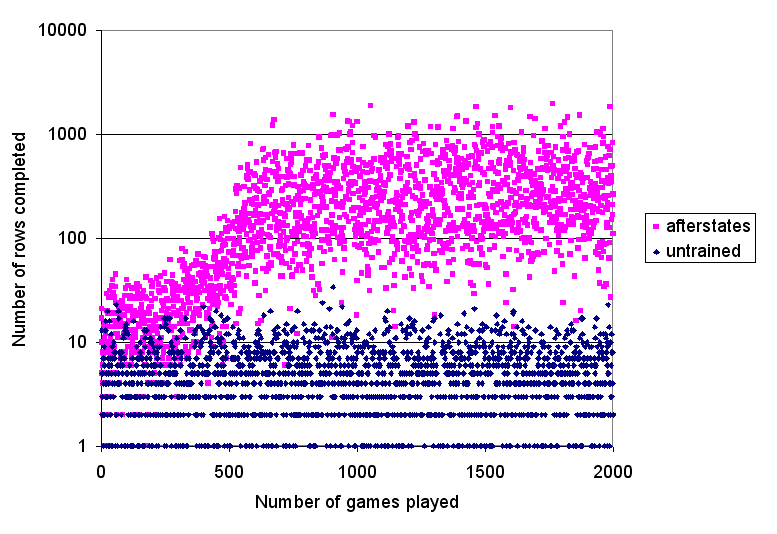
\includegraphics[width=3in]{afterstatesredtet5well.png}
\caption{Afterstates agent in well of width 5}
\label{fig:comparemelax}
\end{figure}

\begin{figure}[h]
\centering
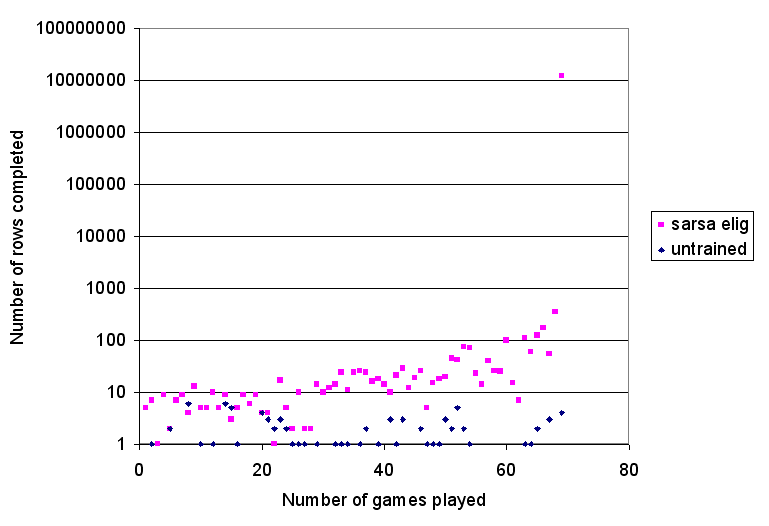
\includegraphics[width=3in]{sarsaeligredtet4well.png}
\caption{Sarsa agent in well of width 4}
\label{fig:comparemelax}
\end{figure}

\begin{figure}[h]
\centering
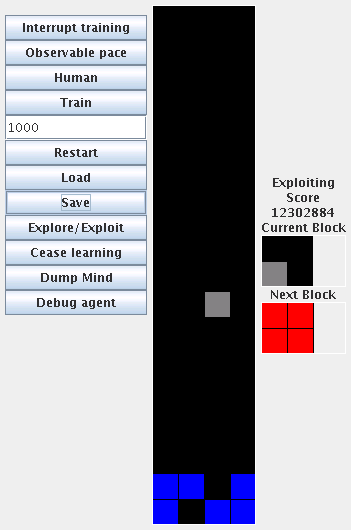
\includegraphics[width=3in]{sarsaelig4term.png}
\caption{Sarsa agent at time of termination}
\label{fig:comparemelax}
\end{figure}

\begin{figure}[h]
\centering
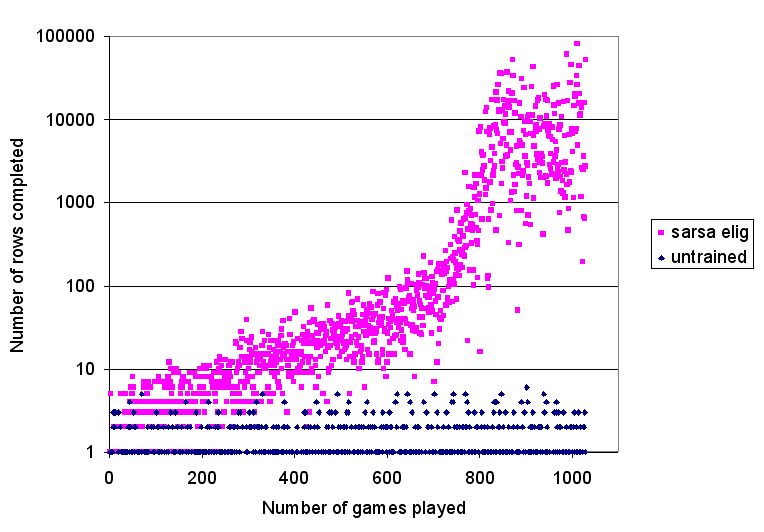
\includegraphics[width=3in]{sarsaeligredtet5well.png}
\caption{Sarsa agent in well of width 5}
\label{fig:comparemelax}
\end{figure}

\chapter{Full Tetris}

\begin{figure}[h]
\centering
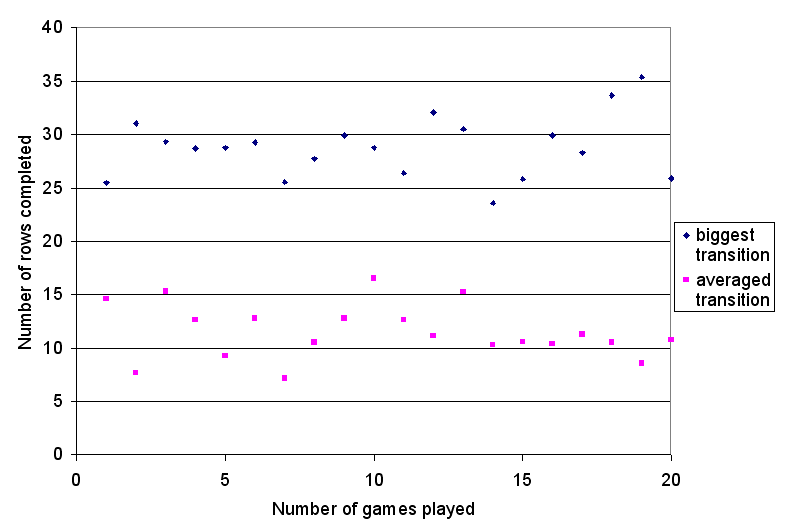
\includegraphics[width=3in]{multisingle.png}
\caption{Contrast between biggest transition and average transition}
\label{fig:comparemelax}
\end{figure}

\begin{figure}[h]
\centering
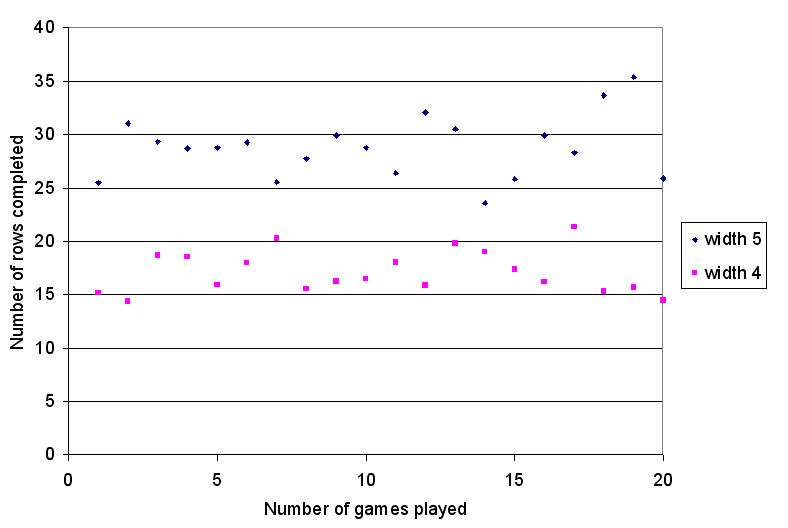
\includegraphics[width=3in]{widthcomparrison.png}
\caption{Comparrison of extendability of subwell sizes with reduced tetrominoes}
\label{fig:comparemelax}
\end{figure}

\begin{figure}[h]
\centering
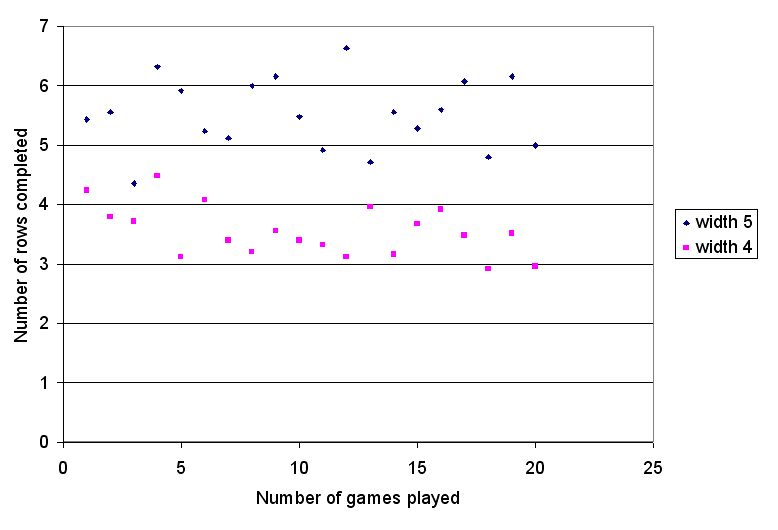
\includegraphics[width=3in]{widthcomparrisonfulltet.png}
\caption{Comparrison of extendability of subwell sizes with standard tetrominoes}
\label{fig:comparemelax}
\end{figure}


\begin{figure}[h]
\centering
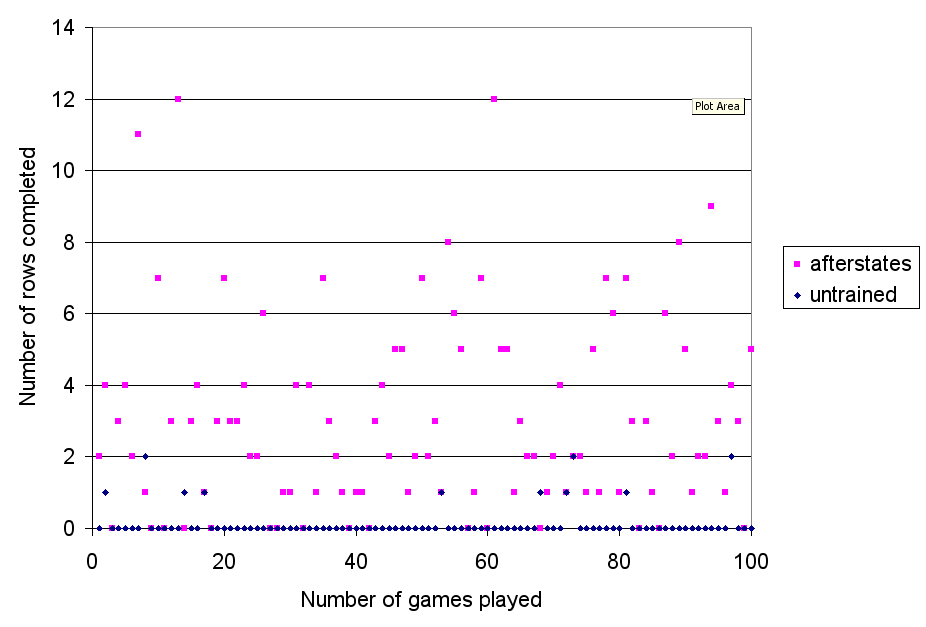
\includegraphics[width=3in]{afterstatesredtetfullwell.png}
\caption{Afterstates agent in full well with red tetrominoes}
\label{fig:comparemelax}
\end{figure}

\begin{figure}[h]
\centering
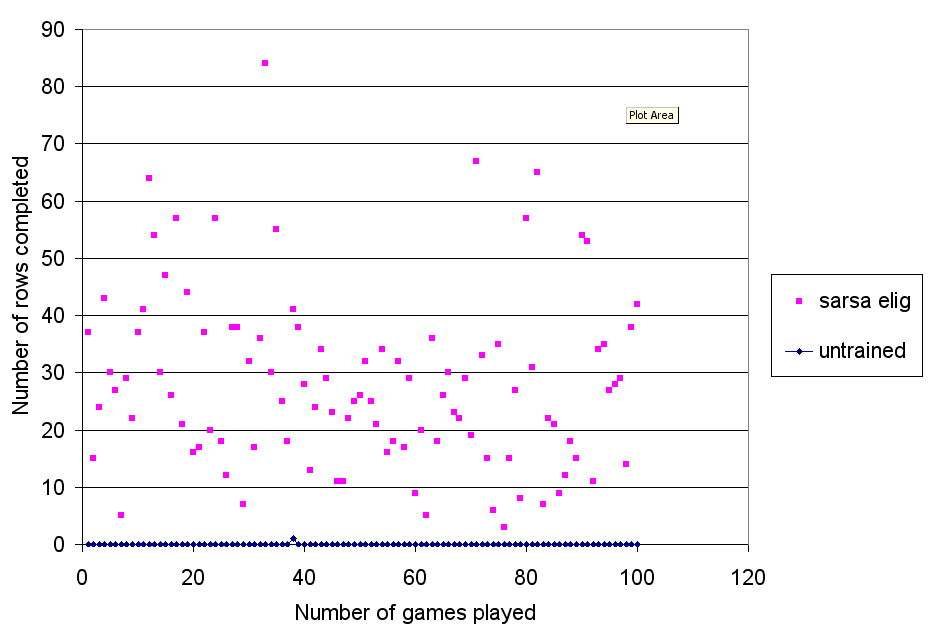
\includegraphics[width=3in]{sarsaeligredtetfullwell.png}
\caption{Sarsa agent in full well with red tetrominoes}
\label{fig:comparemelax}
\end{figure}

\begin{figure}[h]
\centering
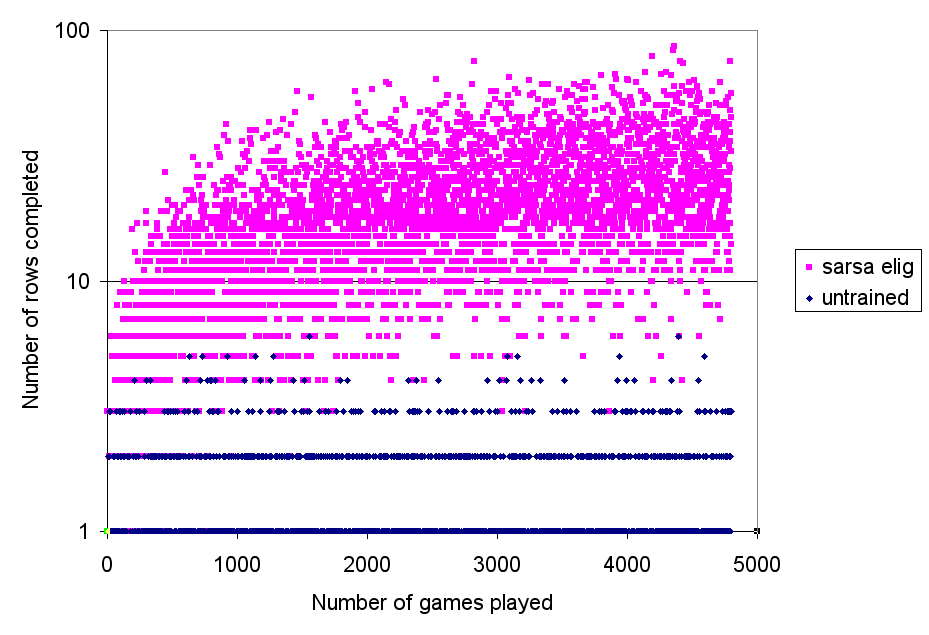
\includegraphics[width=3in]{sarsaeligfulltetredwell.png}
\caption{Sarsa agent in reduced well with full tetrominoes}
\label{fig:comparemelax}
\end{figure}

\begin{figure}[h]
\centering
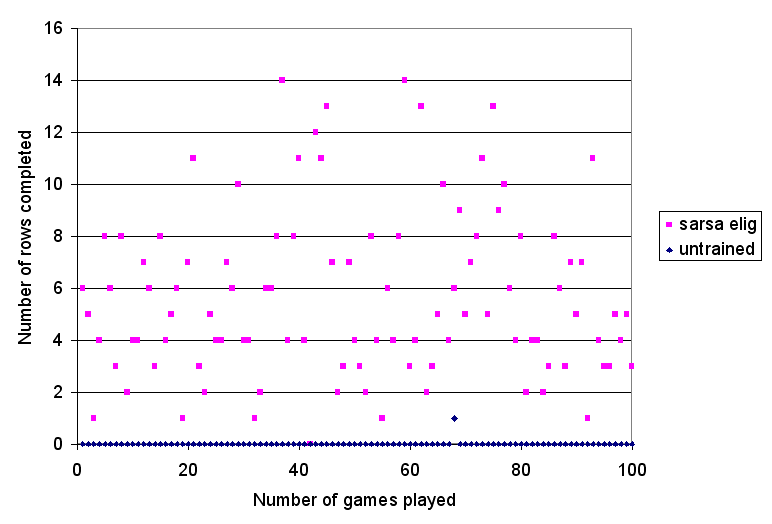
\includegraphics[width=3in]{sarsaeligfulltetfullwell.png}
\caption{Sarsa agent in full well with full tetrominoes}
\label{fig:comparemelax}
\end{figure}

\begin{figure}[h]
\centering
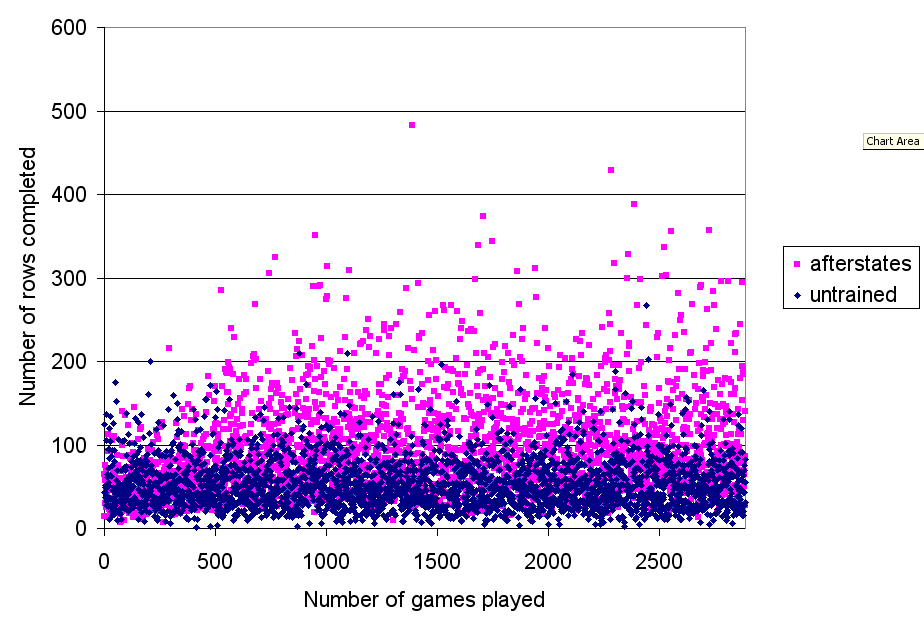
\includegraphics[width=3in]{afterstatesheightredtetfullwell.png}
\caption{Afterstates agent in full well with red tetrominoes}
\label{fig:comparemelax}
\end{figure}

The final step was that of extending our contour playing agent to the full Tetris game.

Although the reduced representation was chosen to be four blocks wide, agents trained in narrow wells developed a policy which favoured easy returns. In narrow wells there is a rapid turnover of rows since 2 blocks on average complete a row. Introducing holes therefore has minor implications as rows have a short lifespan and the obstructing layer is likely to removed in the ensuing block placements. This performance does not scale out to the full representation of the game, where a single introduced hole can devalue a series of successive compact placements and have long term implications.

By extending the width of the reduced well the agent trains within a broader well and tends towards a policy that reflects the policy required in playing the game. We narrowed the well in order to reduce the state space, and every extra unit of width increases the state space by a factor of seven for our contour representation. We therefore seek to strike a balance between increasing the state space and giving the agent access to the environment we want him to eventually solve.

Increasing the well width to five blocks increased the afterstates and sarsa state spaces by a factor of seven, which still kept the statespace feasible although time demanding in their exploration. This also 
 
In discovering possible transitions, the agent previously iterated through every possible positional placement and every orientation of the current tetromino within these placements. In extending the reduced representation to the full game, the agent had to iterate through all the sub-wells comprising the full well and investigate the value of the transitions in the subwells.


\chapter{Conclusions}

The afterstates agent acheived incredibly results when playing within the original subwell. These results were unrealistically high, and dropped off sharply as the well was increased and real time rewards became more intermittant. The afterstates representation neglected the importance of different transitions.

The sarsa player acheived incredible results within the original subwell defined in the state space reduction. The performance was still impressive as the well width was increased, although the required training time greatly increased.

The reducing of the state representation had a greater impact on the afterstates approach, since this approach depends purely on the accuracy of the state information. The extended resolution afforded the sarsa player enabled it to associate a value with the act of transitioning off a state. 

\bibliography{finalwriteup}

\end{document}
